%%%%%%%%%%%%%%%%%%%%%%%%%%%%%%%%%%%%%%%%%
% Programming/Coding Assignment
% LaTeX Template
%
% This template has been downloaded from:
% http://www.latextemplates.com
%
% Original author:
% Ted Pavlic (http://www.tedpavlic.com)
%
% Note:
% The \lipsum[#] commands throughout this template generate dummy text
% to fill the template out. These commands should all be removed when 
% writing assignment content.
%
% This template uses a Perl script as an example snippet of code, most other
% languages are also usable. Configure them in the "CODE INCLUSION 
% CONFIGURATION" section.
%
%%%%%%%%%%%%%%%%%%%%%%%%%%%%%%%%%%%%%%%%%

%----------------------------------------------------------------------------------------
%	PACKAGES AND OTHER DOCUMENT CONFIGURATIONS
%----------------------------------------------------------------------------------------

\documentclass{article}

\usepackage{fancyhdr} % Required for custom headers
\usepackage{lastpage} % Required to determine the last page for the footer
\usepackage{extramarks} % Required for headers and footers
\usepackage[usenames,dvipsnames]{color} % Required for custom colors
\usepackage{graphicx} % Required to insert images
\usepackage{listings} % Required for insertion of code
\usepackage{courier} % Required for the courier font
\usepackage{lipsum} % Used for inserting dummy 'Lorem ipsum' text into the template
\usepackage{url}
\graphicspath{{images/}}

% Margins
\topmargin=-0.45in
\evensidemargin=0in
\oddsidemargin=0in
\textwidth=6.5in
\textheight=9.0in
\headsep=0.25in

\linespread{1.1} % Line spacing

% Set up the header and footer
\pagestyle{fancy}
\lhead{\hmwkAuthorName} % Top left header
\chead{\hmwkClass\ (\hmwkClassInstructor\ \hmwkClassTime): \hmwkTitle} % Top center head
\rhead{\firstxmark} % Top right header
\lfoot{\lastxmark} % Bottom left footer
\cfoot{} % Bottom center footer
\rfoot{Page\ \thepage\ of\ \protect\pageref{LastPage}} % Bottom right footer
\renewcommand\headrulewidth{0.3pt} % Size of the header rule
\renewcommand\footrulewidth{0.4pt} % Size of the footer rule

\setlength\parindent{0pt} % Removes all indentation from paragraphs

%----------------------------------------------------------------------------------------
%	CODE INCLUSION CONFIGURATION
%----------------------------------------------------------------------------------------

\definecolor{MyDarkGreen}{rgb}{0.0,0.4,0.0} % This is the color used for comments
\lstloadlanguages{R} % Load Perl syntax for listings, for a list of other languages supported see: ftp://ftp.tex.ac.uk/tex-archive/macros/latex/contrib/listings/listings.pdf
\lstset{language=R, % Use Perl in this example
        frame=single, % Single frame around code
        basicstyle=\small\ttfamily, % Use small true type font
        breaklines=true,
        keywordstyle=[1]\color{Blue}\bf, % Perl functions bold and blue
        keywordstyle=[2]\color{Purple}, % Perl function arguments purple
        keywordstyle=[3]\color{Blue}\underbar, % Custom functions underlined and blue
        identifierstyle=, % Nothing special about identifiers                                         
        commentstyle=\usefont{T1}{pcr}{m}{sl}\color{MyDarkGreen}\small, % Comments small dark green courier font
        stringstyle=\color{Purple}, % Strings are purple
        showstringspaces=false, % Don't put marks in string spaces
        tabsize=5, % 5 spaces per tab
        %
        % Put standard Perl functions not included in the default language here
        morekeywords={},
        %
        % Put Perl function parameters here
        morekeywords=[2]{on, off, interp},
        %
        % Put user defined functions here
        morekeywords=[3]{test},
       	%
        morecomment=[l][\color{Blue}]{...}, % Line continuation (...) like blue comment
        numbers=left, % Line numbers on left
        firstnumber=1, % Line numbers start with line 1
        numberstyle=\tiny\color{Blue}, % Line numbers are blue and small
        stepnumber=5 % Line numbers go in steps of 5
}

% Creates a new command to include a perl script, the first parameter is the filename of the script (without .pl), the second parameter is the caption
\newcommand{\rscript}[2]{
\begin{itemize}
\item[]\lstinputlisting[caption=#2,label=#1]{#1.R}
\end{itemize}
}

%----------------------------------------------------------------------------------------
%	DOCUMENT STRUCTURE COMMANDS
%	Skip this unless you know what you're doing
%----------------------------------------------------------------------------------------

% Header and footer for when a page split occurs within a problem environment
\newcommand{\enterProblemHeader}[1]{
\nobreak\extramarks{#1}{#1 continued on next page\ldots}\nobreak
\nobreak\extramarks{#1 (continued)}{#1 continued on next page\ldots}\nobreak
}

% Header and footer for when a page split occurs between problem environments
\newcommand{\exitProblemHeader}[1]{
\nobreak\extramarks{#1 (continued)}{#1 continued on next page\ldots}\nobreak
\nobreak\extramarks{#1}{}\nobreak
}

\setcounter{secnumdepth}{0} % Removes default section numbers
\newcounter{homeworkProblemCounter} % Creates a counter to keep track of the number of problems

\newcommand{\homeworkProblemName}{}
\newenvironment{homeworkProblem}[1][Problem \arabic{homeworkProblemCounter}]{ % Makes a new environment called homeworkProblem which takes 1 argument (custom name) but the default is "Problem #"
\stepcounter{homeworkProblemCounter} % Increase counter for number of problems
\renewcommand{\homeworkProblemName}{#1} % Assign \homeworkProblemName the name of the problem
\section{\homeworkProblemName} % Make a section in the document with the custom problem count
\enterProblemHeader{\homeworkProblemName} % Header and footer within the environment
}{
\exitProblemHeader{\homeworkProblemName} % Header and footer after the environment
}

\newcommand{\problemAnswer}[1]{ % Defines the problem answer command with the content as the only argument
\noindent\framebox[\columnwidth][c]{\begin{minipage}{0.98\columnwidth}#1\end{minipage}} % Makes the box around the problem answer and puts the content inside
}

\newcommand{\homeworkSectionName}{}
\newenvironment{homeworkSection}[1]{ % New environment for sections within homework problems, takes 1 argument - the name of the section
\renewcommand{\homeworkSectionName}{#1} % Assign \homeworkSectionName to the name of the section from the environment argument
\subsection{\homeworkSectionName} % Make a subsection with the custom name of the subsection
\enterProblemHeader{\homeworkProblemName\ [\homeworkSectionName]} % Header and footer within the environment
}{
\enterProblemHeader{\homeworkProblemName} % Header and footer after the environment
}

\newcommand{\quotes}[1]{``#1''}
%----------------------------------------------------------------------------------------
%	NAME AND CLASS SECTION
%----------------------------------------------------------------------------------------

\newcommand{\hmwkTitle}{Homework\ \#3} % Assignment title
\newcommand{\hmwkDueDate}{9/16/2017} % Due date
\newcommand{\hmwkClass}{Applied Data Mining} % Course/class
\newcommand{\hmwkClassTime}{Online} % Class/lecture time
\newcommand{\hmwkClassInstructor}{Instructor: Hasan Kurban} % Teacher/lecturer
\newcommand{\hmwkAuthorName}{Keith Hickman} % Your name

%----------------------------------------------------------------------------------------
%	TITLE PAGE
%----------------------------------------------------------------------------------------

\title{
\vspace{2in}
\textmd{\textbf{\hmwkClass:\ \hmwkTitle}}\\
\normalsize\vspace{0.1in}\small{Due\ on\ \hmwkDueDate}\\
\vspace{0.1in}\large{\textit{\hmwkClassInstructor\ }}
\vspace{3in}
}

\author{\textbf{\hmwkAuthorName}}
\date{\today} % Insert date here if you want it to appear below your name

%----------------------------------------------------------------------------------------

\begin{document}

\maketitle

%----------------------------------------------------------------------------------------
%	TABLE OF CONTENTS
%----------------------------------------------------------------------------------------

%\setcounter{tocdepth}{1} % Uncomment this line if you don't want subsections listed in the ToC

%\newpage
%\tableofcontents
\newpage


In this homework, you will work with 
Ionosphere Data Set  to answer some questions regarding  Principal Component Analysis (PCA), exploratory data analysis and k-means clustering.  Here is the beginning of an R session that allows us to read this data from the web into our local R session:
\begin{verbatim}
> install.packages("data.table")
> library(data.table)
> install.packages("curl")
> mydata <- fread("https://archive.ics.uci.edu/ml/machine-learning-databases/
                   ionosphere/ionosphere.data")
             
\end{verbatim}


%%%%%%%%%%%%%%%%%%%%%%%%%%%%%%%%%%

%PROBLEM 1
%%%%%%%%%%%%%%%%%%%%%%%%%%%%%%%%%%
\begin{homeworkProblem}
For the Ionosphere Data Set, answer the following questions:
\subsection{Discussion of Data}
Briefly describe this data set--what is its purpose?  How should it be used? What are the kinds of data it's using?
This dataset records observations of radar signatures of free electrons in the ionosphere.  The set's purpose is to measure whether the radar signatures were detecting the electrons or passing through.
\subsection{R Code}
 Using R, show code that answers the following questions:
\begin{enumerate} 
\item How many entries are in the data set? A: There are 351 observations $\ldots$
\rscript{sb}{Sample R Script With Highlighting}

\item How many unknown or missing data are in the data set?  $\ldots$
A: There are no missing variables in the dataset.  
\rscript{sb}{Sample R Script With Highlighting}

\begin{verbatim}
35  Variables      351  Observations
----------------------------------------------------------------------------------------------------
V1 
       n  missing distinct     Info      Sum     Mean      Gmd 
     351        0        2     0.29      313   0.8917   0.1936 

             ...
\end{verbatim}

\item Create a bar plot  of 1st, 2nd, 35th variables. Label the plots properly. Discuss the distribution of values \textit{e.g.}, are uniform, skewed, normal.  Place images of these bar plots into the document.   Show the R code that you used below and discussion below that. 
\rscript{sb1}{Sample R Script With Highlighting}

\subsection{Discussion of  Bar Plots}
A:  Unfortunately, the dataset documentation is somewhat sparse.  For variables V1 and V2, it seems there is a highly skewed distribution.  V1 is 300 observations of 1 vs. 50 of 0.  V2 is homogenous.  Would that count as a uniform distribution? 
Either way, there is not much information contained in V2.  V35 is the class or target variable, and is skewed toward toward the positive class - 1.  $\ldots$
\subsection{Bar Plots}
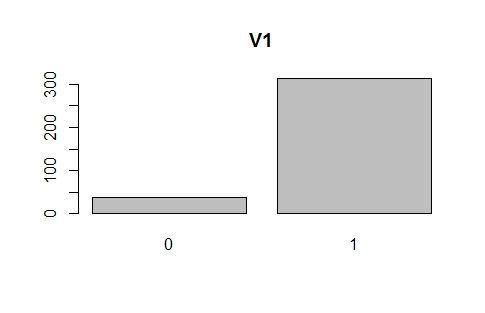
\includegraphics{v1bar.jpeg}
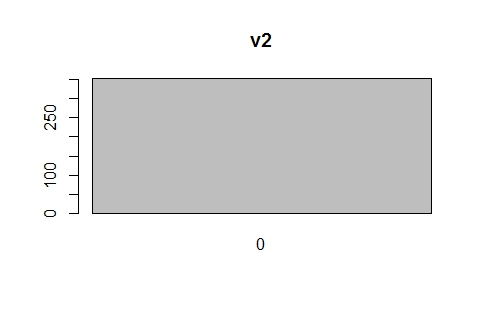
\includegraphics{v2bar.jpeg}
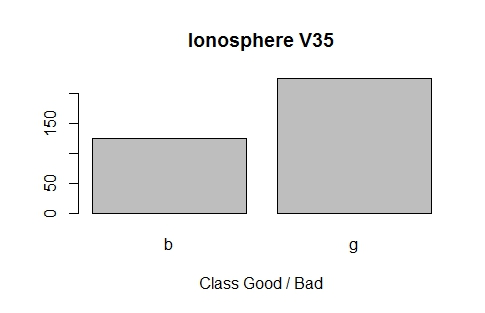
\includegraphics{v35bar.jpeg}

\item Make a scatter plots of [$V22, V20$] and [$V1,V2$] variables and color the data points with the class variable [$V35$]. Discuss the plots, i.e., do you observe any relationships between variables?

\rscript{sb2}{Sample R Script With Highlighting}
\subsection{Discussion of  Scatter Plots}
I was able to produce a basic scatter plot of the X, Y variables V20 and V22 respectively.  I was not able to use the ggplot library's color feature to color by the target variable V35.  
I kept getting error messages indicating that V35 wasn't a valid color variable.  However, the text states on pg. 104 that R should convert those into integers.  The relationship between the two variablesV20 and V22 is linear.  The relationship seems to be centered around zero $\ldots$
\subsection{Scatter Plots}
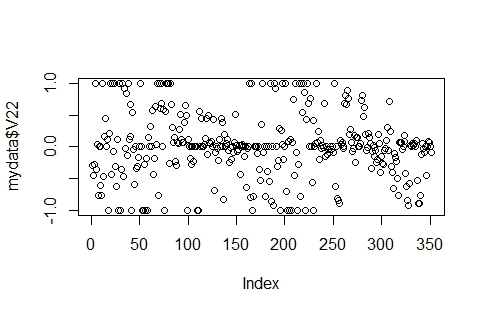
\includegraphics{scatter1.jpeg}
\end{enumerate}
\end{homeworkProblem}


%%%%%%%%%%%%%%%%%%%%%%%%%%%%%%%%%

%PROBLEM 2
%%%%%%%%%%%%%%%%%%%%%%%%%%%%%%%%%%
\begin{homeworkProblem}
 In this question,  you will run $k$-means clustering algorithm against Ionosphere data set. The  input  data for $k$-means is $mydata[,-35]$ -- removing the class variable since this is a clustering task.
\subsection{R Code}
 Using R, show code that answers the following questions:
\begin{enumerate} 

\item Run  \quotes{Lloyd, Forgy and Hartigan-Wong's} heuristic algorithms for $k$-means and report total within sum of squared error (SSE) for $k=2$ and  $nstart = 50$. Compare the results?i.e., which/why is better? Discuss  $nstart$ parameter. Show the R code that you used below and discussion and results below that.
\rscript{sb4}{Sample R Script With Highlighting}
\subsection{Total SSE}

A: The total within SSE is 2419.365.  Note: I was confused by the reference to Lloyd, Forgy, and Hartigan-Wong.  I couldn't find it anywhere in the text.  Were they the progentors of heuristics for k-means in R?  

\subsection{Discussion of  $\textbf{nstart}$ and Results}
Adjusting n-start upwards increases the number of iterations the k-means algorithm would go through, thereby potentially decreasing the SSE.  $\ldots$


\item  Elbow method is a technique used to decide  optimal cluster number. The code below  gives a plot of total SSE for $k=1,\ldots,10$. Discuss the elbow technique, i.e., what would be the optimal $k$ based on the plot, can optimal $k$ always be identified by elbow method?

\begin{verbatim}
> k_max <- 10
#total SSE
> tsse <- sapply(1:k_max, 
+               function(k){kmeans(mydata, k, nstart=30,iter.max = 12 )
                                    $tot.withinss})
> tsse
 [1] 3243.103 2419.365 2193.320 1998.581
  1889.717 1806.150 1737.575 1668.753 1617.829 1550.105
> plot(1:k_max, tsse,
+      type="b", pch = 20, frame = FALSE, 
+      xlab="Number of clusters k",
+      ylab="Total within-clusters sum of squares")
> 	
\end{verbatim}

\subsection{Discussion of  Results}
I noticed that the biggest increase in SSE included within clusters is obviously from 1 to 2, then diminishes with each additional cluster.  How do we determine the number of optimal clusters?  I would consider the number of meaningful clusters as the main driver e.g. the number that we could act upon.  If I had a customer segmentation problem, I would want to know the number of groups I could reasonably segment my customer base into.  

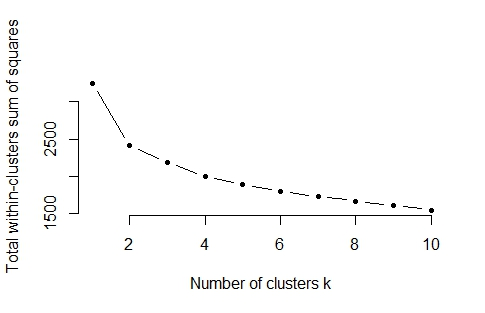
\includegraphics{optimalcluster.jpeg}
\end{enumerate} 
\end{homeworkProblem}


%%%%%%%%%%%%%%%%%%%%%%%%%%%%%%%%%

%PROBLEM 3
%%%%%%%%%%%%%%%%%%%%%%%%%%%%%%%%%%
\begin{homeworkProblem}
 Use Principal Component Analysis (PCA) over Ionosphere Data Set to answer the below questions. You may want to use either \quotes{\textit{princomp()}} or \quotes{\textit{prcomp()}} functions in R. In this question,  remove the 2nd (all $0$s) and 35th variable (class variable) before using PCA.
 
 
 \begin{verbatim}
> mydata <- mydata[,-35]
> mydata <- mydata[,-2]
> dim(mydata)
[1] 351  33
> mydata.pca <- prcomp(mydata, scale =TRUE)
\end{verbatim}


\subsection{R Code}
 Using R, show code that answers the following questions:
\begin{enumerate} 

\item Make a scatter plot of PC1 and PC2 (the first and second principal components).  Discuss principal components? What is PC1 and PC2? Show the R code that you used below and the scatter plot and discussion below that
\rscript{sb5}{Sample R Script With Highlighting}
\subsection{Scatter Plot}

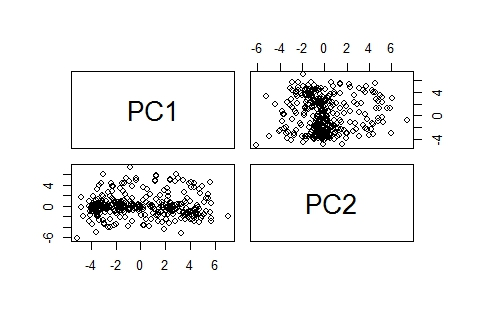
\includegraphics{pca12.jpeg}

\subsection{Discussion of  Principal Components}
PCA 1 and 2 are linear combinations of the variables in the mydata dataset.  They each explain a decreasing amount of the variance in the dataset. Here, the PC1 explains 26 percent of the variance, followed by 12 percent, down to 1 and 2 percent.
There are roughly 11 or 12 PCs that I would include to explain most of the variance while still reducing dimensionality. 


\item  You can observe the loadings as follows (using \textit{prcomp() function}):

 \begin{verbatim}
>mydata.pca$rotation 
\end{verbatim}
 Discuss loadings in PCA?i.e., how are principal components and original variables of the data (mydata) related? (loadings(mydata.pca) if  \textit{princomp()} is used)
The original variables differ significantly in their contributions to the PCA.  

\item  Scree plot is among the most popular methods to decide optimal dimension number.

 \begin{verbatim}
> plot(mydata.pca, type = "l") 
> screeplot(mydata.pca)
\end{verbatim}

What is the optimal dimension number ($d$) for this data set? How much of the variation is kept with your optimal $d$? Discuss the results.
A:  If I look at the elbow plot, I would estimate that three (3) PCs would be the optimum number of dimensions, as more than three decreases the percent of variance explained by a significant amount.  
However, when I look at the scree plot, I would increase the number of PCs to five (5) to accomodate the max variance.   
\end{enumerate} 


\end{homeworkProblem}


%----------------------------------------------------------------------------------------

\end{document}